\chapter{研究背景和现状}{
{
\let\cleardoublepage\relax
}

\section{研究背景}

\subsection{容器化环境简介}

容器是应用程序的标准单元,它将应用程序的代码及其所有依赖项打包在内,以便在不同的硬件和软件环境中都可以正确执行,解决了兼容性问题,实现应用程序的可移植性\citep{whatcontainer}。相比起虚拟机,容器无需包含整个操作系统,因此容器是轻量化的,开销低\citep{Schenker2023}。由于不包含操作系统,因此容器需共享主机上的操作系统内核,这基于资源隔离技术实现\citep{Jain2020}。这些资源隔离技术包括:

\begin{itemize}
    \item 命名空间机制。将容器的网络、文件系统挂载、用户组等资源与主机隔离,使容器不能看到主机上的资源,而只能看到容器内部的资源。
    \item 更改根目录机制。将容器内的根目录限制在容器内部,避免容器读、写或执行主机上的文件。
    \item 控制组(Control Group,cgroup)机制。限制了容器可使用主机上的处理器、内存等资源的配额。
\end{itemize}

为了提高应用程序的可用性和稳定性,通常采用分布式体系结构。对于容器化的应用程序而言,则相应地采用分布式的容器化结构,这些运行不同容器的主机构成容器化集群。为了支撑容器化集群的管理,需要容器编排工具以提供资源配额、调度、负载均衡、运行状况检查、容错、自动缩放、自动修复等功能。

图~\ref{fig:orchestration}~展示了一个部署在云上的容器化集群的分层架构\citep{Casalicchio2019}。

\begin{figure}[t]
    \centering
    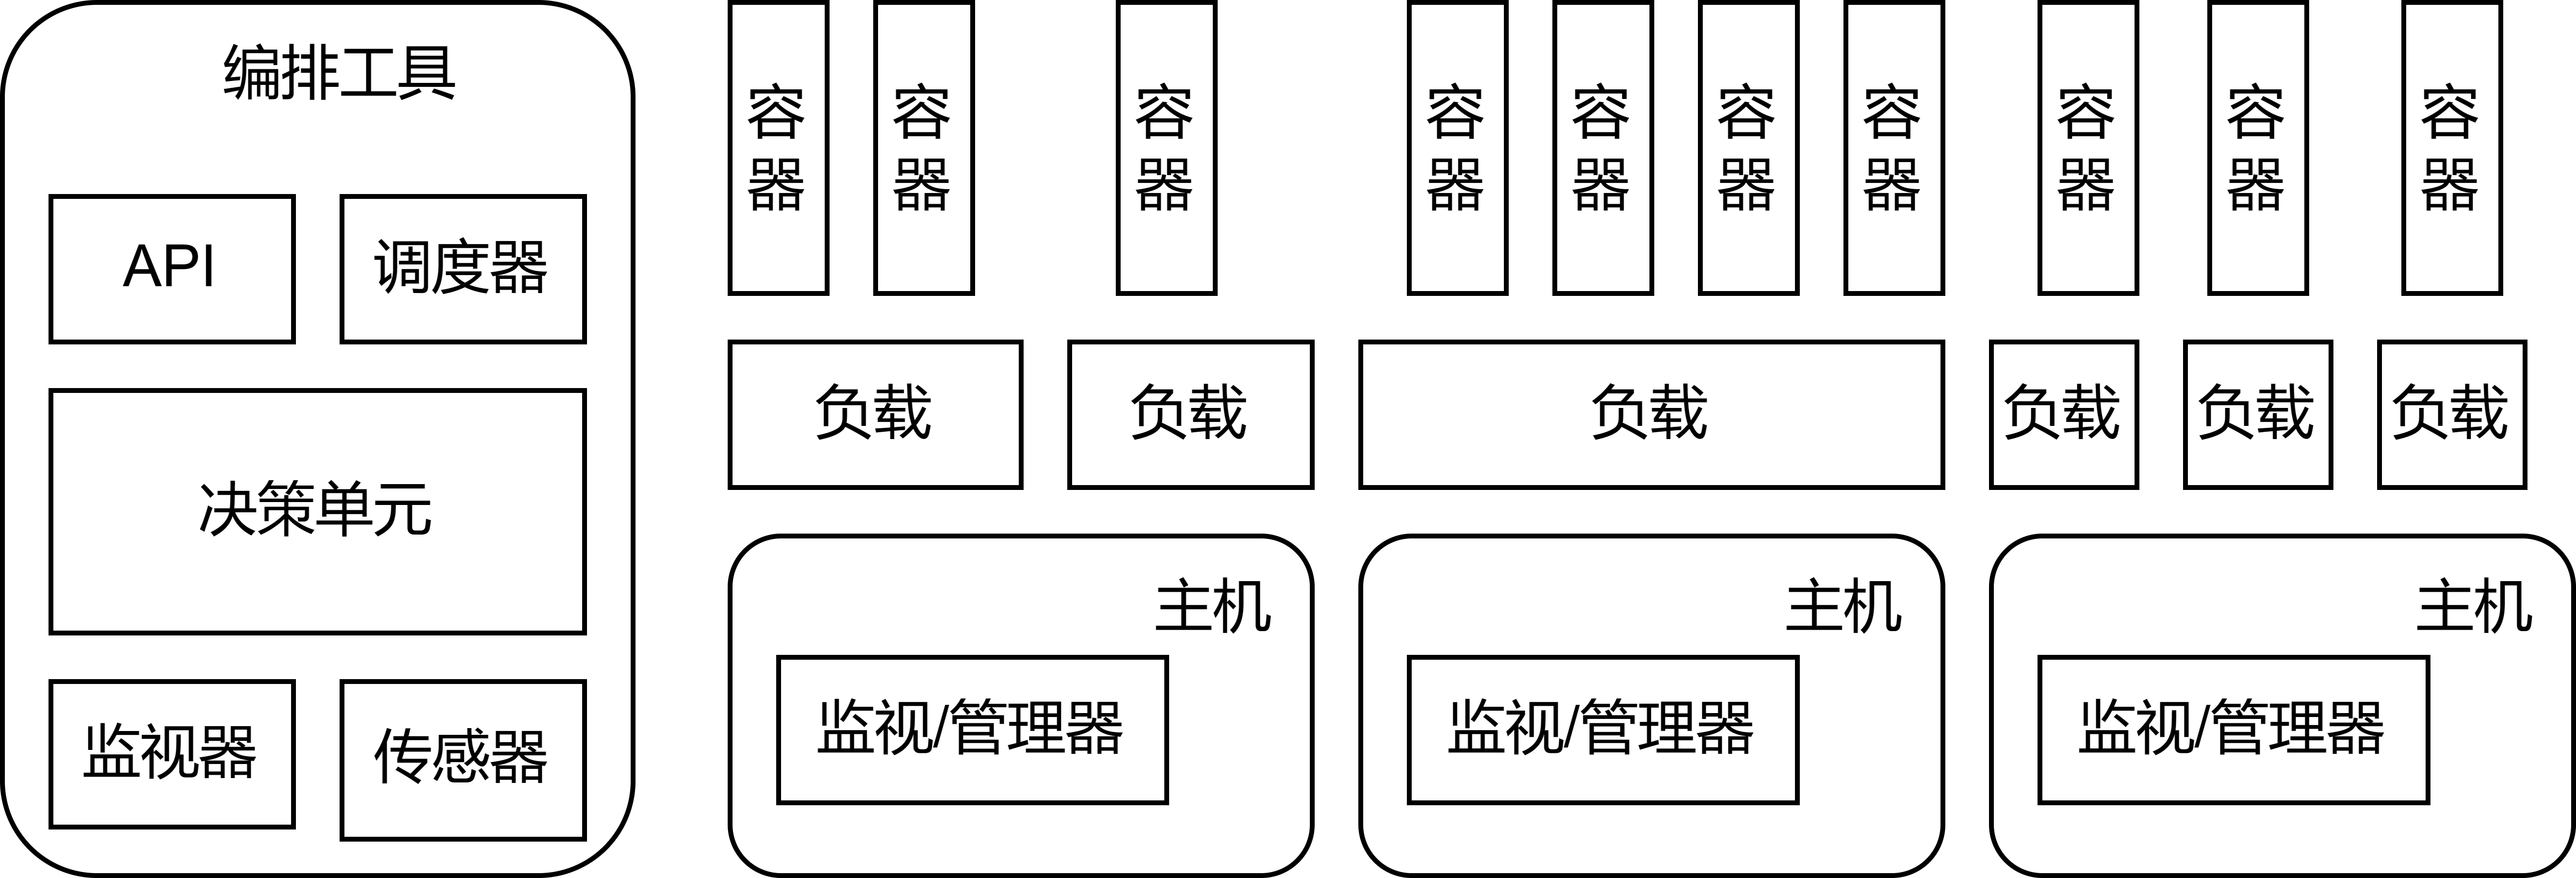
\includegraphics[width=1.00\textwidth]{orchestration}
    \bicaption{\enspace 容器化集群的架构}{\enspace The architecture of a containerized cluster}
    \label{fig:orchestration}

\end{figure}

容器化集群中的调度通常以负载为单位进行,单个负载中包含一个或多个容器,由编排工具的调度器调度到主机上。主机上均部署了监视器,将该主机的运行情况传输至编排工具的传感器中,以便编排工具检查主机的运行情况和工作载荷等。编排工具上也部署了监视器,负责检查负载及其包含的容器的运行状况(通常通过网络请求等方式探测)。编排工具的决策单元将根据用户设定的规则,执行自动缩放、自动修复等任务,具体任务通过主机上的管理器实施。编排工具还提供应用程序接口(Application Programming Interface,API),以便调整配置和管理集群中的资源。

\subsection{容器化环境下的安全问题}

由于容器化环境中包含多种多样的组件,因此其攻击面十分广泛,任何一个组件存在缺陷都会对容器化环境造成威胁。这些攻击面如图~\ref{fig:attack-vector}~所示\citep{liz2018}。

\begin{figure}[t]
    \centering
    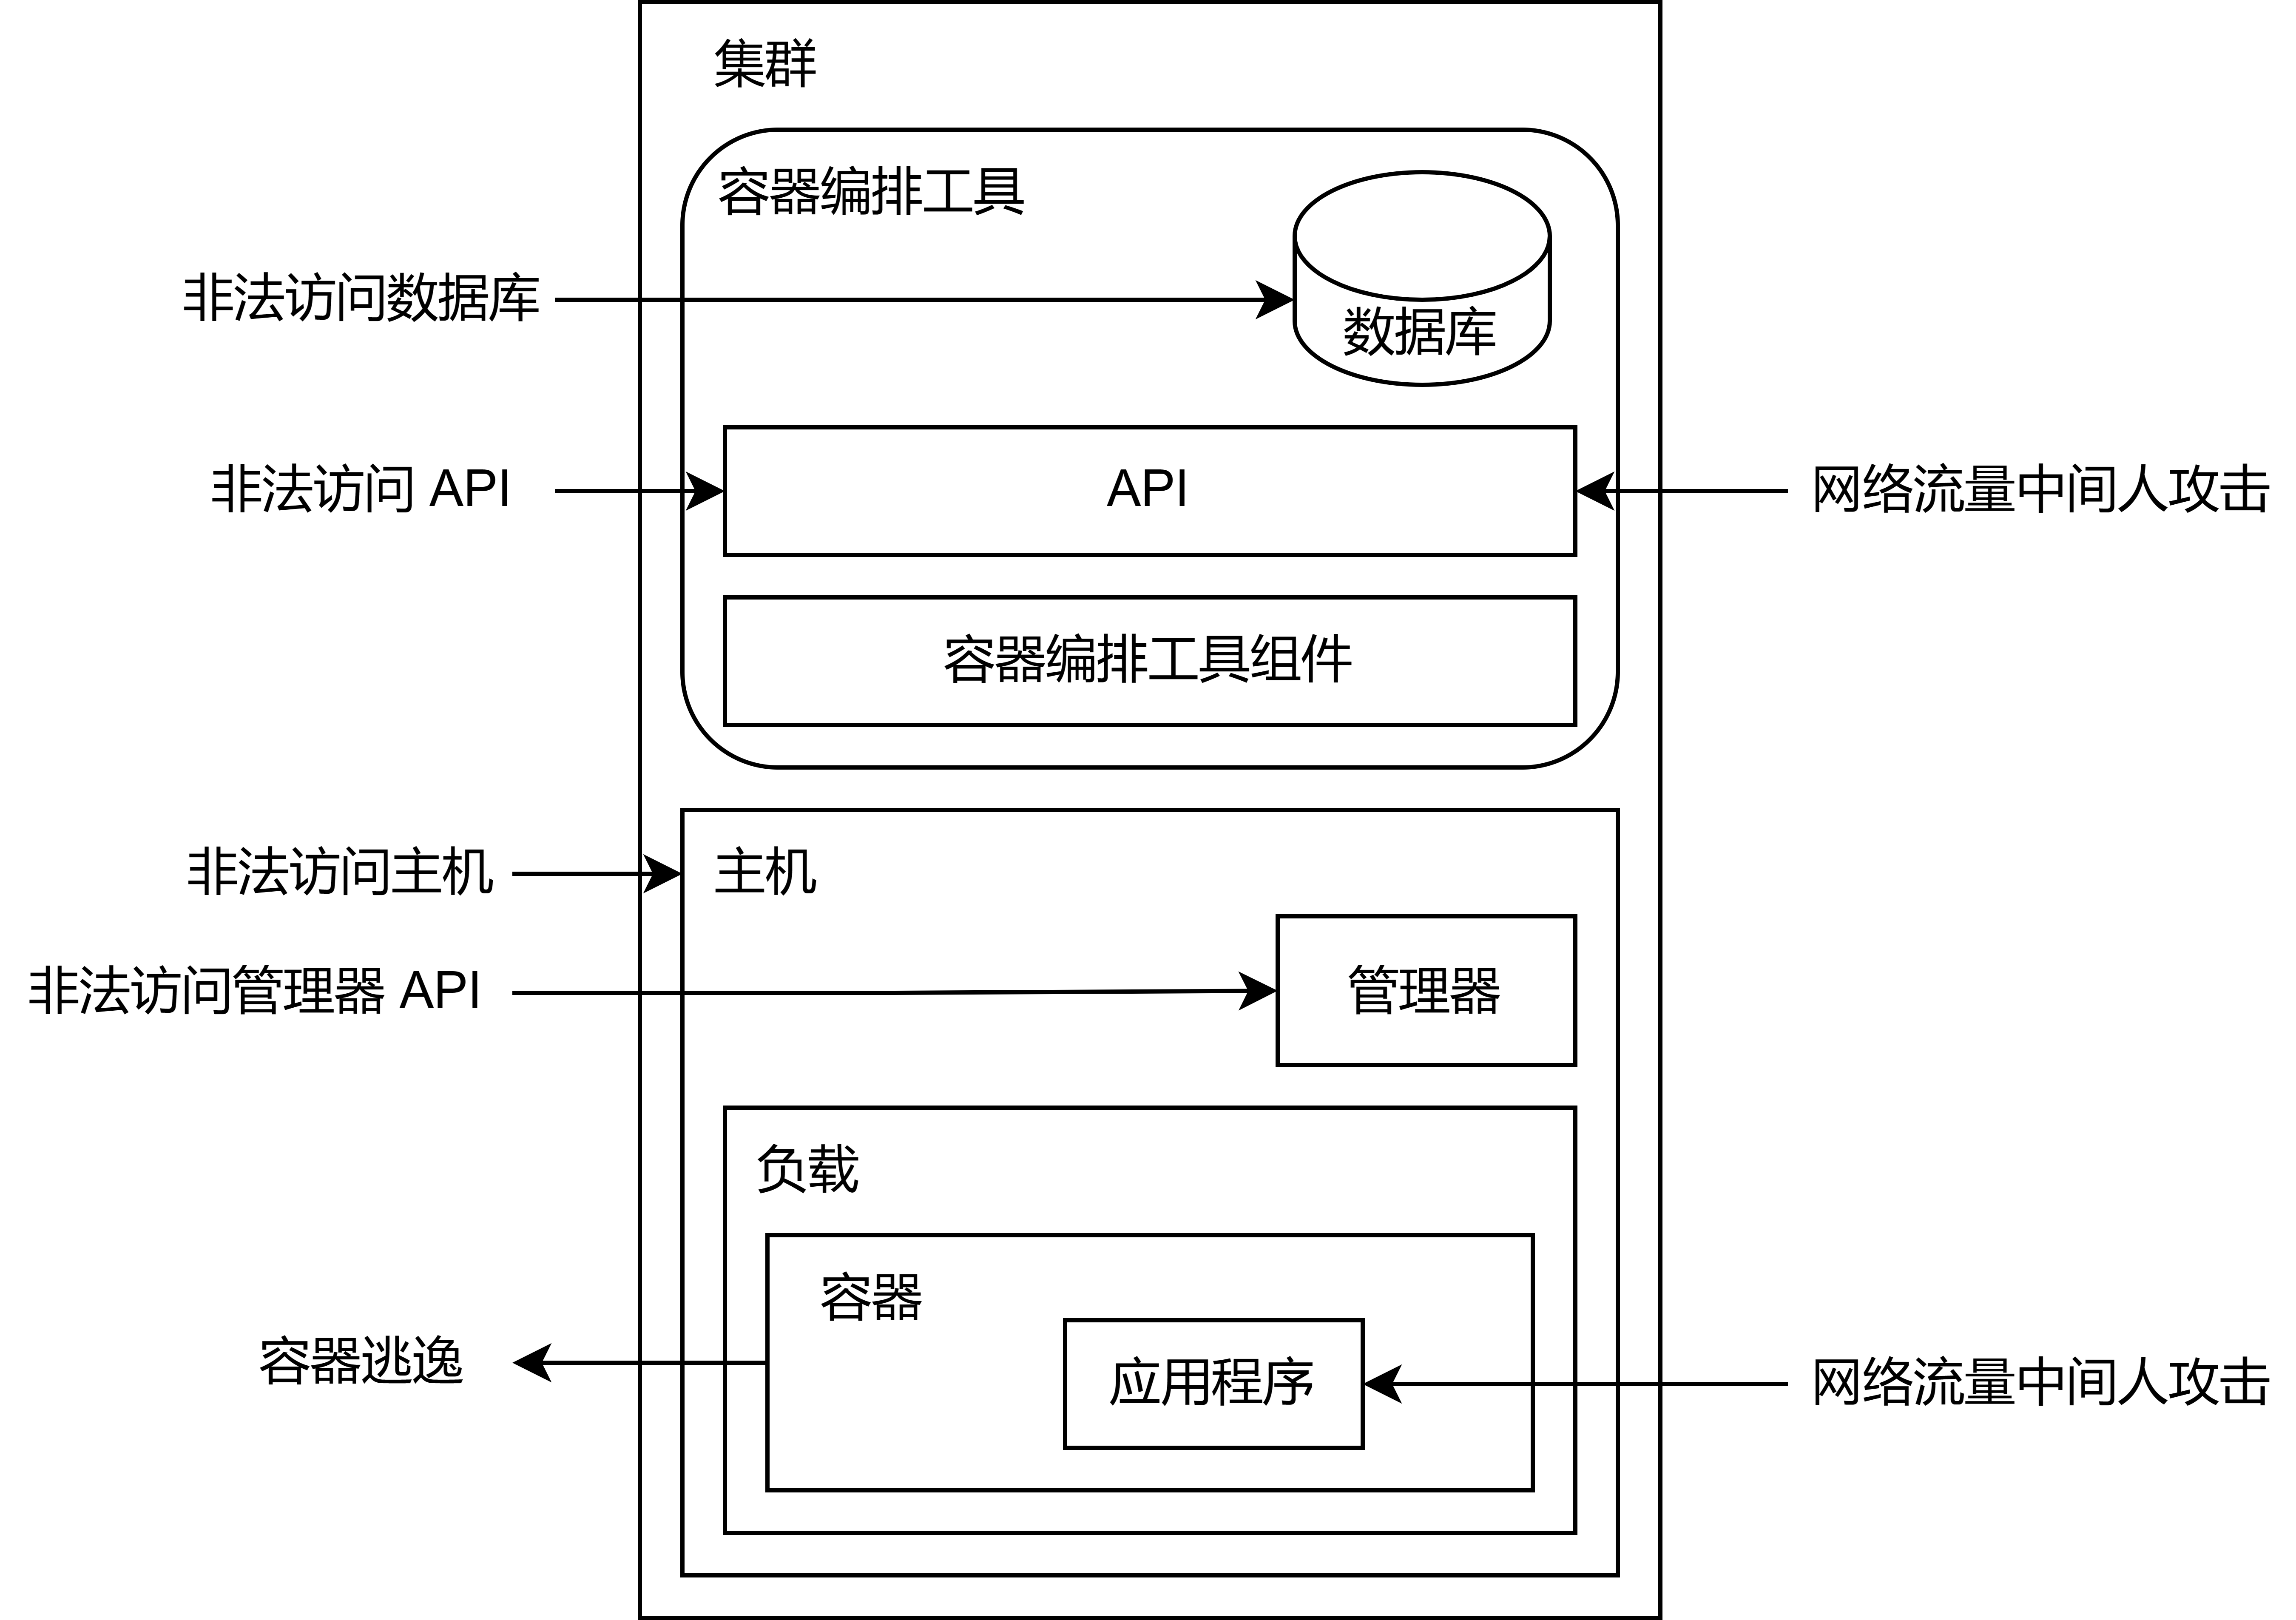
\includegraphics[width=1.00\textwidth]{attack-vector}
    \bicaption{\enspace 容器化集群的攻击面\citep{liz2018}}{\enspace Attack vectors of containerized clusters\citep{liz2018}}
    \label{fig:attack-vector}

\end{figure}

这些攻击面与 OWASP 基金会公布的网络应用程序十大安全风险\citep{owasp}相吻合。这些安全风险包括\citep{liz2020}:

\begin{itemize}
    \item 访问控制配置不当。由于容器通常在 Linux 操作系统上运行,而只有根用户才能使用资源隔离技术,所以容器默认情况下在根用户下运行,这就导致可能产生容器逃逸的风险。此外,在容器化集群中,访问控制配置不当还会产生 API 被滥用,导致数据泄露或系统无法正常运行的风险。
    \item 加密信息泄露。虽然容器编排工具的 API 默认仅允许加密流量,但开发者仍需自行为应用程序的流量加密负责。若进行了明文传输,则会导致应用程序存在被攻击的风险,从而使容器化集群陷入威胁。
    \item 注入漏洞。注入漏洞可能存在于各种 API 请求中,因此容器编排工具、主机上的管理器和应用程序都面临风险。
    \item 不安全的设计。若容器化集群未经过最小特权原则、纵深防御原则、零信任原则和安全开放原则设计,则会面临威胁。
    \item 安全配置错误。在容器化集群中,使用环境变量传递密钥会导致这些密钥通过日志泄露,威胁集群的安全。
    \item 易受攻击和过时的组件。若容器使用过时的应用程序版本,则该容器可能会包含漏洞,导致攻击者入侵到容器中。
    \item 身份认证失败。攻击者通过撞库、弱密码、盗窃会话标识符等方式登录到应用程序中,使容器化集群面临风险。
    \item 软件和数据完整性丢失。攻击者通过污染公开的应用程序源发起供应链攻击,当集群中的容器使用这类应用程序时,导致集群面临威胁。
    \item 不充分的监控和日志。平均而言,违规行为需要近 200 天才能被识别\citep{liz2020}。通过详细记录网络入站和出站等容器事件,可以显著减少这种情况。
    \item 服务器端请求伪造。这会面临内部的端口扫描、元数据和敏感数据泄露、内部服务被破坏等威胁。
\end{itemize}

因此,通过充分地监控并记录网络连接日志,可以减少容器化环境中存在的威胁。本研究基于网络流量展开横向移动检测的研究。

\section{现有横向移动检测方法}

为检测横向移动,可运用多种技术和方法。通常,可以从网络流量、端点行为、用户行为和威胁情报四方面进行检测:

\begin{itemize}
    \item 基于网络流量的检测:可通过异常的端口扫描、大量的数据传输、使用非标准协议的通信等方面进行检测;
    \item 基于端点行为的检测:可通过异常的进程创建、异常的文件访问、异常的注册表修改等方面进行检测;
    \item 基于用户行为的检测:可通过登录异常账户、访问异常的资源、执行异常的操作等方面进行检测;
    \item 基于威胁情报的检测:攻击者通常会使用已知的工具和技术进行横向移动。通过分析威胁情报,可以识别出攻击者可能使用的工具和技术,并提前进行防御。
\end{itemize}

\subsection{基于端点行为和威胁情报的检测}

Latte\citep{liu2018latte} 利用 Windows 系统和安全事件构建网络连接图,当网络中发生远程文件执行(常规检测场景)或者检测到被攻击的节点(取证分析场景)时,可利用该网络连接图找到可能的横向移动路径。然而,该方法与 Windows 系统深度绑定,无法用于容器化环境中的检测。

\subsection{基于用户行为的检测}

Log2vec\citep{liu2019log2vec}通过对用户操作日志(如登录、访问网页、发送邮件、打开文件等)建模成图,生成各节点的嵌入向量后,通过一种聚类方法,将较小的聚类认定为异常操作。在容器化场景中,没有用户行为的信息可以利用,TCP/IP 流量中也无相关用户行为信息。不过,在容器化集群中,各 Pod 的日志或许可用于横向移动检测,这有待未来的工作。

\subsection{基于网络流量的检测}

大多数横向移动检测方法通过网络流量来检测横向移动,但它们仅关注由登录活动产生的网络流量。这方法基于一个关键的假设:攻击者通常执行横向移动来访问最初的受害者无法访问的机器。

这些方法检测横向移动的模型各不相同,但都采取了将网络流量日志建模成登录图的方法,其中图的节点代表计算机,边代表计算机之间产生的流量。这些方法如表~\ref{tab:recent}~所示。

\begin{table}[t]
    \bicaption{\enspace 现有横向移动检测方法}{\enspace Recent lateral movement detection methods}
    \label{tab:recent}
    \centering
    \footnotesize% fontsize
    \setlength{\tabcolsep}{4pt}% column separation
    \renewcommand{\arraystretch}{1.2}%row space 
    \begin{tabular}{ccccccccc}
        \hline
        方法 & 机器学习模型 & 数据集 & 效果\\
        \hline
        Kent 等人\citep{kent2015authentication} & 无 & LANL\citep{kent-2015-cyberdata1} & 检测率28\% 误报率0.13\%\\
        Siadati 等人\citep{siadati2017detecting} & 无 & 私有数据集 & 检测率82\% 误报率0.3\%\\
        Bowman 等人\citep{bowman2020detecting} & Node2vec\citep{grover2016node2vec}、Logistic & LANL\citep{kent-2015-cyberdata1} & 检测率85\% 误报率0.9\%\\
        Hopper\citep{ho2021hopper} & 无 & 私有数据集 & 检测率94.5\% 误报率0.12\%\\
        Euler\citep{king2023euler} & GCN\citep{kipf2016semi}、GRU\citep{cho2014learning} & LANL\citep{kent-2015-cyberdata1} & 检测率86.1\% 误报率0.57\% AUC 99.12\%\\
        Jbeil\citep{khoury2023jbeil} & TGN\citep{rossi2020temporal} & LANL\citep{kent-2015-cyberdata1} & AUC 99.31\%\\
        \hline
    \end{tabular}
\end{table}

可以看到,这些方法采用的数据集及其评估指标不尽相同,并且均在企业网络等非容器化环境下进行横向移动检测,未对容器化场景进行研究。

Kent 等人\citep{kent2015authentication}通过提取图的特征后,使用 Logistic 回归模型检测横向移动。该方法提取图的特征包括图的节点数、边数、图形密度等。这种提取方法在图神经网络流行的今天看起来已经十分老旧,实现起来比较繁琐,并且效果欠佳。

Siadati 等人\citep{siadati2017detecting}统计挖掘了若干个最常通信的用户、源计算机、目标计算机三元组$\left<U,S,D\right>$,对于一个登录记录$\left<u,s,d\right>$,若该登录记录符合其中一个三元组即$u \in U, s \in S, d \in D$,则认为该登录是正常的;否则认定为横向移动。该方法的优点是可解释性强;缺点是其三元组的挖掘方式较低效,需要枚举所有可能的 $\left<U,S,D\right>$,用时较长。

Bowman 等人\citep{bowman2020detecting}是首个采用了机器学习的方法,它采用 Node2vec 模型学习登录图并生成各节点的嵌入向量,对于每条登录记录,计算该登录记录中两个节点的逐元素乘积并通过 Logistic 模型预测该登录记录为横向移动的概率。该方法的优点是采用了机器学习的方法,比先前的方法更有效地提取图的特征;缺点是它将登录图视为静态的,未能体现网络的动态性,对于原本正常但后来被感染的计算机,难以检出其横向移动行为。

Hopper\citep{ho2021hopper}则对路径之间的因果关系进行了深入研究。该方法定义了登录记录之间因果关系的聚合方法,对于两条登录记录 $L_1=\left<s_1, d_1\right>$ 和 $L_2=\left<s_2, d_2\right>$,若 $L_1$ 发生在 $L_2$ 之前 24 小时之内,并且 $L_1$ 的目的计算机等于 $L_2$ 的源计算机即 $d_1=s_2$,那么 $L_1$ 与 $L_2$ 呈``因果关系'',$L_1$ 是 $L_2$ 的原因。多条因果登录记录通过上述规则聚合为登录路径。Hopper 检查登录路径上的用户信息,若用户信息发生了变化,则视为横向移动;若用户信息没有发生变化,则不是横向移动。然而,由于因果关系聚合方法不够精确,一条登录记录的原因可能是多条登录记录之一而无法准确判断,对于这类不明确且可能存在用户信息变化的登录路径,Hopper 通过历史登录记录和历史告警记录推断发生横向移动的概率。该方法的优点是考虑了登录路径的时序关系,缺点是其登录路径规则聚合方法较繁琐,且需排除多种白名单情况(例如跳板机、新机器等),导致其准确率还有待提高。此外,该方法在私有的 Dropbox 数据集上完成,其检测结果无法与其他方法直接对比。

Euler\citep{king2023euler}采用类似 GCRN\citep{seo2018gcrn} 模型的方式将图深度学习网络和循环神经网络堆叠起来。该方法首先根据设定的时间间隔,划分时间片,为每个时间片生成一张登录图;然后,使用图深度学习网络为登录图中每个节点生成嵌入向量;接着将这些向量输入到循环神经网络中,得到下一时刻节点嵌入向量的预测;再对两个节点的嵌入向量进行点积,就得到这两个节点存在登录记录的概率,将概率较低者判定为横向移动。图深度学习网络为 GCN、GraphSAGE\citep{hamilton2017inductive}、GAT\citep{velivckovic2017graph} 任选其一,循环神经网络为 GRU、LSTM\citep{hochreiter1997long}、None(即使用恒等映射)任选其一。该方法的优点是考虑了网络的动态性,并结合了深度学习方法,使其准确性大大提高;缺点是需要划分时间片,使每个时间片内部的时序关系丢失。

Jbeil\citep{khoury2023jbeil}是企业网络内检测横向移动的最新方法。它引用 TGN 模型,避免了时间片的划分。该方法由图特征提取模块、记忆模块和嵌入模块两方面构成。对于图特征提取模块,模型计算每个节点每日的特征,例如该节点当日用户登录数、节点当日登录计算机数等。对于节点的记忆模块,模型按时间顺序处理每条登录记录,更新登录记录源节点和目的节点的记忆向量,节点记忆向量的更新采用循环神经网络。对于节点的嵌入模块,模型枚举节点的每一个历史邻居节点,将节点当时的记忆向量、节点当时的特征、历史邻居节点当时的记忆向量、历史邻居节点当时的特征通过注意力函数得到节点当前的嵌入向量。最后,模型将两个节点的嵌入向量经过解码器,得到这两个节点存在边的概率,将概率较低者判定为横向移动。该方法的优点是无需划分时间片,因此不会丢失时间数据,这使得其准确率大大提高。

上述方法的共同缺点在于,它们均采用了图的链路预测方式来检测横向移动,即判断两个节点存在登录记录的概率。然而,在容器化场景中,没有相应的登录记录信息可用,因为攻击者入侵到集群中时并非是根据任何人的身份信息登录到集群中,而是利用负载的漏洞等,通过远程代码执行的方式入侵到集群中。此外,容器化集群的 API 服务器虽然负责进行身份认证和鉴权,但涉及集群内部操作时,API 服务器主要鉴定的是负载、主机的身份,而非人的身份。

在容器化集群中,使用网络流量信息来检测横向移动时,也不能简单地采用图的链路预测方法。因为这类方法仅判断边的存在性,而没有考虑边上的特征;但在容器化集群中,边上的特征即网络流量的特征发挥非常重要的作用。这将在第~\ref{sec:analyze}~节中详细描述。

\section{容器化环境中的横向移动检测技术路线}

横向移动是网络入侵攻击的一个阶段,因此横向移动检测是入侵检测系统的一类。基于网络流量的入侵检测系统通常有如下可行的技术路线\citep{ahmad2021network, darban2022deep}:

\begin{itemize}
    \item 传统机器学习方法。包括决策树、K-最近邻、K-均值、支持向量机等。这些方法实现简单,运行速度快,但准确率低。
    \item 循环神经网络方法。循环神经网络用于预测一个序列在下一个时刻的值,当预测值与实际值误差较大时,判定为攻击。循环神经网络的变体包括 GRU、LSTM 等,解决梯度消失导致模型无法捕获长距离依赖关系的问题。此外,基于自注意力机制的 Transformer\citep{vaswani2017attention} 模型也可用于取代循环神经网络,因为 Transformer 可并行处理序列,同时仍然保持模型的性能。
    \item 自动编码器。自动编码器由编码器和解码器构成,编码器将输入压缩为隐向量,解码器则将隐向量还原至原来的维度,试图重现原来的输入,然后再重现值与输入对比,误差较大者视为攻击。
    \item 生成对抗网络。生成对抗网络中通常包含生成器和判别器,生成器用于生成与输入尽可能相似的样本,判别器用于尽可能准确地将生成器生成的样本与输入区分开来。通过这种对抗训练方法,可以提高生成器重现输入样本和判别器判断异常样本的准确性。
\end{itemize}

近年来,有许多工作关注上述这几种技术路线。

USAD\citep{audibert2020usad} 使用两个自动编码器 $AE_{1}$、$AE_{2}$ 进行对抗训练。这两个自动编码器共享同一个编码器,但各自有不同的解码器。在训练阶段,对于输入 $W$,首先生成其重现值 $AE_{1}(W)$、$AE_{2}(W)$,然后再将 $AE_{1}(W)$ 重新输入到编码器 $AE_{2}$ 中,得到 $AE_{2}(AE_{1}(W))$。训练时,$AE_{1}$ 使 $AE_{1}(W)$、$AE_{2}(AE_{1}(W))$ 尽可能接近 $W$,$AE_{2}$ 使 $AE_{2}(W)$ 尽可能接近 $W$,$AE_{2}(AE_{1}(W))$ 尽可能远离 $W$。在测试阶段,对 $AE_{1}(W)$ 与 $AE_{2}(AE_{1}(W))$ 和 $W$ 的误差作加权平均来判断异常。通过对抗训练的方式,第二个编码器对异常更加敏感,以便提高检测率。

OmniAnomaly\citep{su2019robust} 是变分自动编码器与循环神经网络的结合。该模型由编码器和解码器两部分组成。编码器接收输入 $\mathbf{x}_t$ 后,经过循环神经网络得到 $\mathbf{e}_t$,再将 $\mathbf{e}_t$ 经过归一化流得到隐向量 $\mathbf{z}_t$。归一化流的核心是可逆变换,可以将已转换的样本变换回原始空间。解码器则接收隐向量 $\mathbf{z}_t$,经过循环神经网络得到 $\mathbf{d}_t$,再将 $\mathbf{d}_t$ 变换回 $\hat{\mathbf{x}}_t$。最后,计算$\hat{\mathbf{x}}_t$与$\mathbf{x}_t$的误差,误差较大者发出警报。

MAD-GAN\citep{li2019mad} 则采用了生成对抗网络结构,包含基于 LSTM-RNN 结构的生成器和基于 LSTM-RNN 结构的判别器。在训练阶段,训练样本与生成器生成的样本一同输入至判别器中,由判别器判断样本是否来源于真实数据。通过训练,使生成器生成的样本尽可能接近真实样本,而判别器尽可能准确地判断样本是否真实。在检测阶段,将测试样本输入至判别器中,得到判别分数;同时将生成器生成的样本与测试样本作差,得到误差分数,最后将误差分数与判别分数作加权平均,得到异常分数,较高者发出警报。

TranAD\citep{tuli2022tranad} 的结构与 USAD 类似,但使用了 Transformer 作为自动编码器模型。通过 Transformer 的自注意力机制,模型的准确率得以提升。

这些方法为本研究提供了有益的思路,基于循环神经网络、自动编码器、对抗训练、Transformer 的方法有助于检测网络流量中的异常,从而检测横向移动行为。

\section{现有的数据集}

在横向移动检测领域,最常用的数据集是 LANL\citep{kent-2015-cyberdata1} 数据集。它是企业内部网络 58 天内各类事件的集合,包括 Windows 身份验证事件、进程事件、网络流量事件和 DNS 事件,并记录了红队的身份验证活动,被广泛用于网络攻击检测。数据集规模较大,包含 12 425 个用户、17 684 台计算机、62 974 个进程和 1 648 275 307 个事件。此外,Laprade 等人提出了 PicoDomain 数据集\citep{laprade2020picodomain}。该数据集是通过模拟的方式生成的,它记录了更详细的事件,包括网络流量、身份认证、DHCP 协议、DNS 协议、文件、HTTP 协议、SSL 协议等,但其规模较小,仅包括 7 台计算机。然而,上述两个数据集是在企业网络内部收集的基于主机事件的数据集,而不是在容器化集群中收集的基于网络流量的数据集,因此不适用于本文所做的研究。

Flora 等人\citep{floraevaluating}总结了近年来可用的入侵检测数据集,其中与容器相关的数据集仅有 Kubernetes-dataset\citep{sever2023kubernetes}、CB-DS\citep{el2022contextualizing} 和 LID-DS\citep{grimmer2019modern},但 CB-DS 和 LID-DS 均记录单台主机上的系统调用信息,而不是容器集群中的网络流量信息。单台主机上的系统调用信息无法适用于由多台主机构成的容器集群;此外,Sever 等人\citep{sever2022empirical}指出,基于网络流量的方法比基于系统调用的方法具有更高的性能。因此,这两个数据集不适用于本文所做的研究。

另一方面,与网络流量相关的数据集有 CIC-IDS-2017\citep{sharafaldin2018toward}、CSE-CIC-IDS-2018\citep{csecicids2018},它们包含了所有 TCP/IP 流的统计特征。但是,这些数据集一是并不在容器化场景下,二是没有针对横向移动场景来研究。这些数据集在一个企业网络环境中收集,包含 SQL 注入、暴力攻击、心脏出血等攻击场景,但不包含具有侦察、立足、横向移动等阶段的完整的攻击链。因此,这两个数据集也不适用于本文所做的研究。

本文将使用 Kubernetes-dataset 作为数据集进行后续研究。

\subsection{Kubernetes-dataset 数据集}
\label{sec:dataset}

Kubernetes-dataset \citep{sever2023kubernetes} 数据集由土耳其中东科技大学(Middle East Technical University)在自建的容器化集群中收集。数据集的收集环境见表~\ref{tab:dataset-environment}。

\begin{table}[t]
    \bicaption{\enspace Kubernetes-dataset 收集环境}{\enspace Kubernetes-dataset collection environment}
    \label{tab:dataset-environment}
    \centering
    \footnotesize% fontsize
    \setlength{\tabcolsep}{4pt}% column separation
    \renewcommand{\arraystretch}{1.2}%row space 
    \begin{tabular}{lcccccccc}
        \hline
        计算机数量 & 2\\
        Pod 数量 & 6\\
        计算机操作系统 & Ubuntu 22.04\\
        Kubernetes 版本 & 1.20.0\\
        containerd 版本 & 1.6.0\\
        Docker 版本 & 20.10.6\\
        CNI 插件 & Kube-OVN\citep{kube-ovn}\\
        部署的服务 & Grafana、InfluxDB、Node-RED\\
        \hline
    \end{tabular}
\end{table}

数据集包含良性流量和 10 类攻击流量的标注,其中,7 类标注中,每类标注对应一个漏洞的利用;剩余 3 类标注对应一个攻击场景。该攻击场景分为三个步骤:

\begin{enumerate}
\item 侦察阶段。攻击者使用 OWASP ZAP\citep{zap} 先被动扫描,然后主动扫描容器化环境中的 Node-RED\citep{nodered} 服务,以收集有利于攻击的信息。
\item 初始攻击阶段。攻击者利用已注入到 Node-RED 中的远程代码执行漏洞,获取到了命令行终端,然后通过负载中的服务账户获取凭据。该服务账户具有新建容器的特权。
\item 横向移动阶段。攻击者利用获取到的服务账户凭据创建了一个新的负载,并将主机上的根目录挂载到负载中。最后,使用 chroot 命令,将命令行终端的根目录切换到主机上的根目录,从而完成了由负载到主机的横向移动过程。
\end{enumerate}

数据集使用 Kube-OVN 进行子网搭建。该工具将在计算机上创建 ovn0 网卡,Pod 与主机通信和 Pod 与外部网络通信的流量将流经该网卡。使用 Tcpdump 捕获两台计算机上的网络流量,并使用 CICFlowMeter\citep{engelen2021troubleshooting} 对流量中的 TCP 流进行聚合。%网络的拓扑结构如图~\ref{fig:networking-1}~所示。

数据集的相关统计信息如表~\ref{tab:dataset-metadata}~所示。本文将基于该数据集攻击场景,选取良性流和标注为``横向移动''的流进行后续研究。选取的流共有 26 758 个。

% \begin{figure}[!htbp]
%     \centering
%     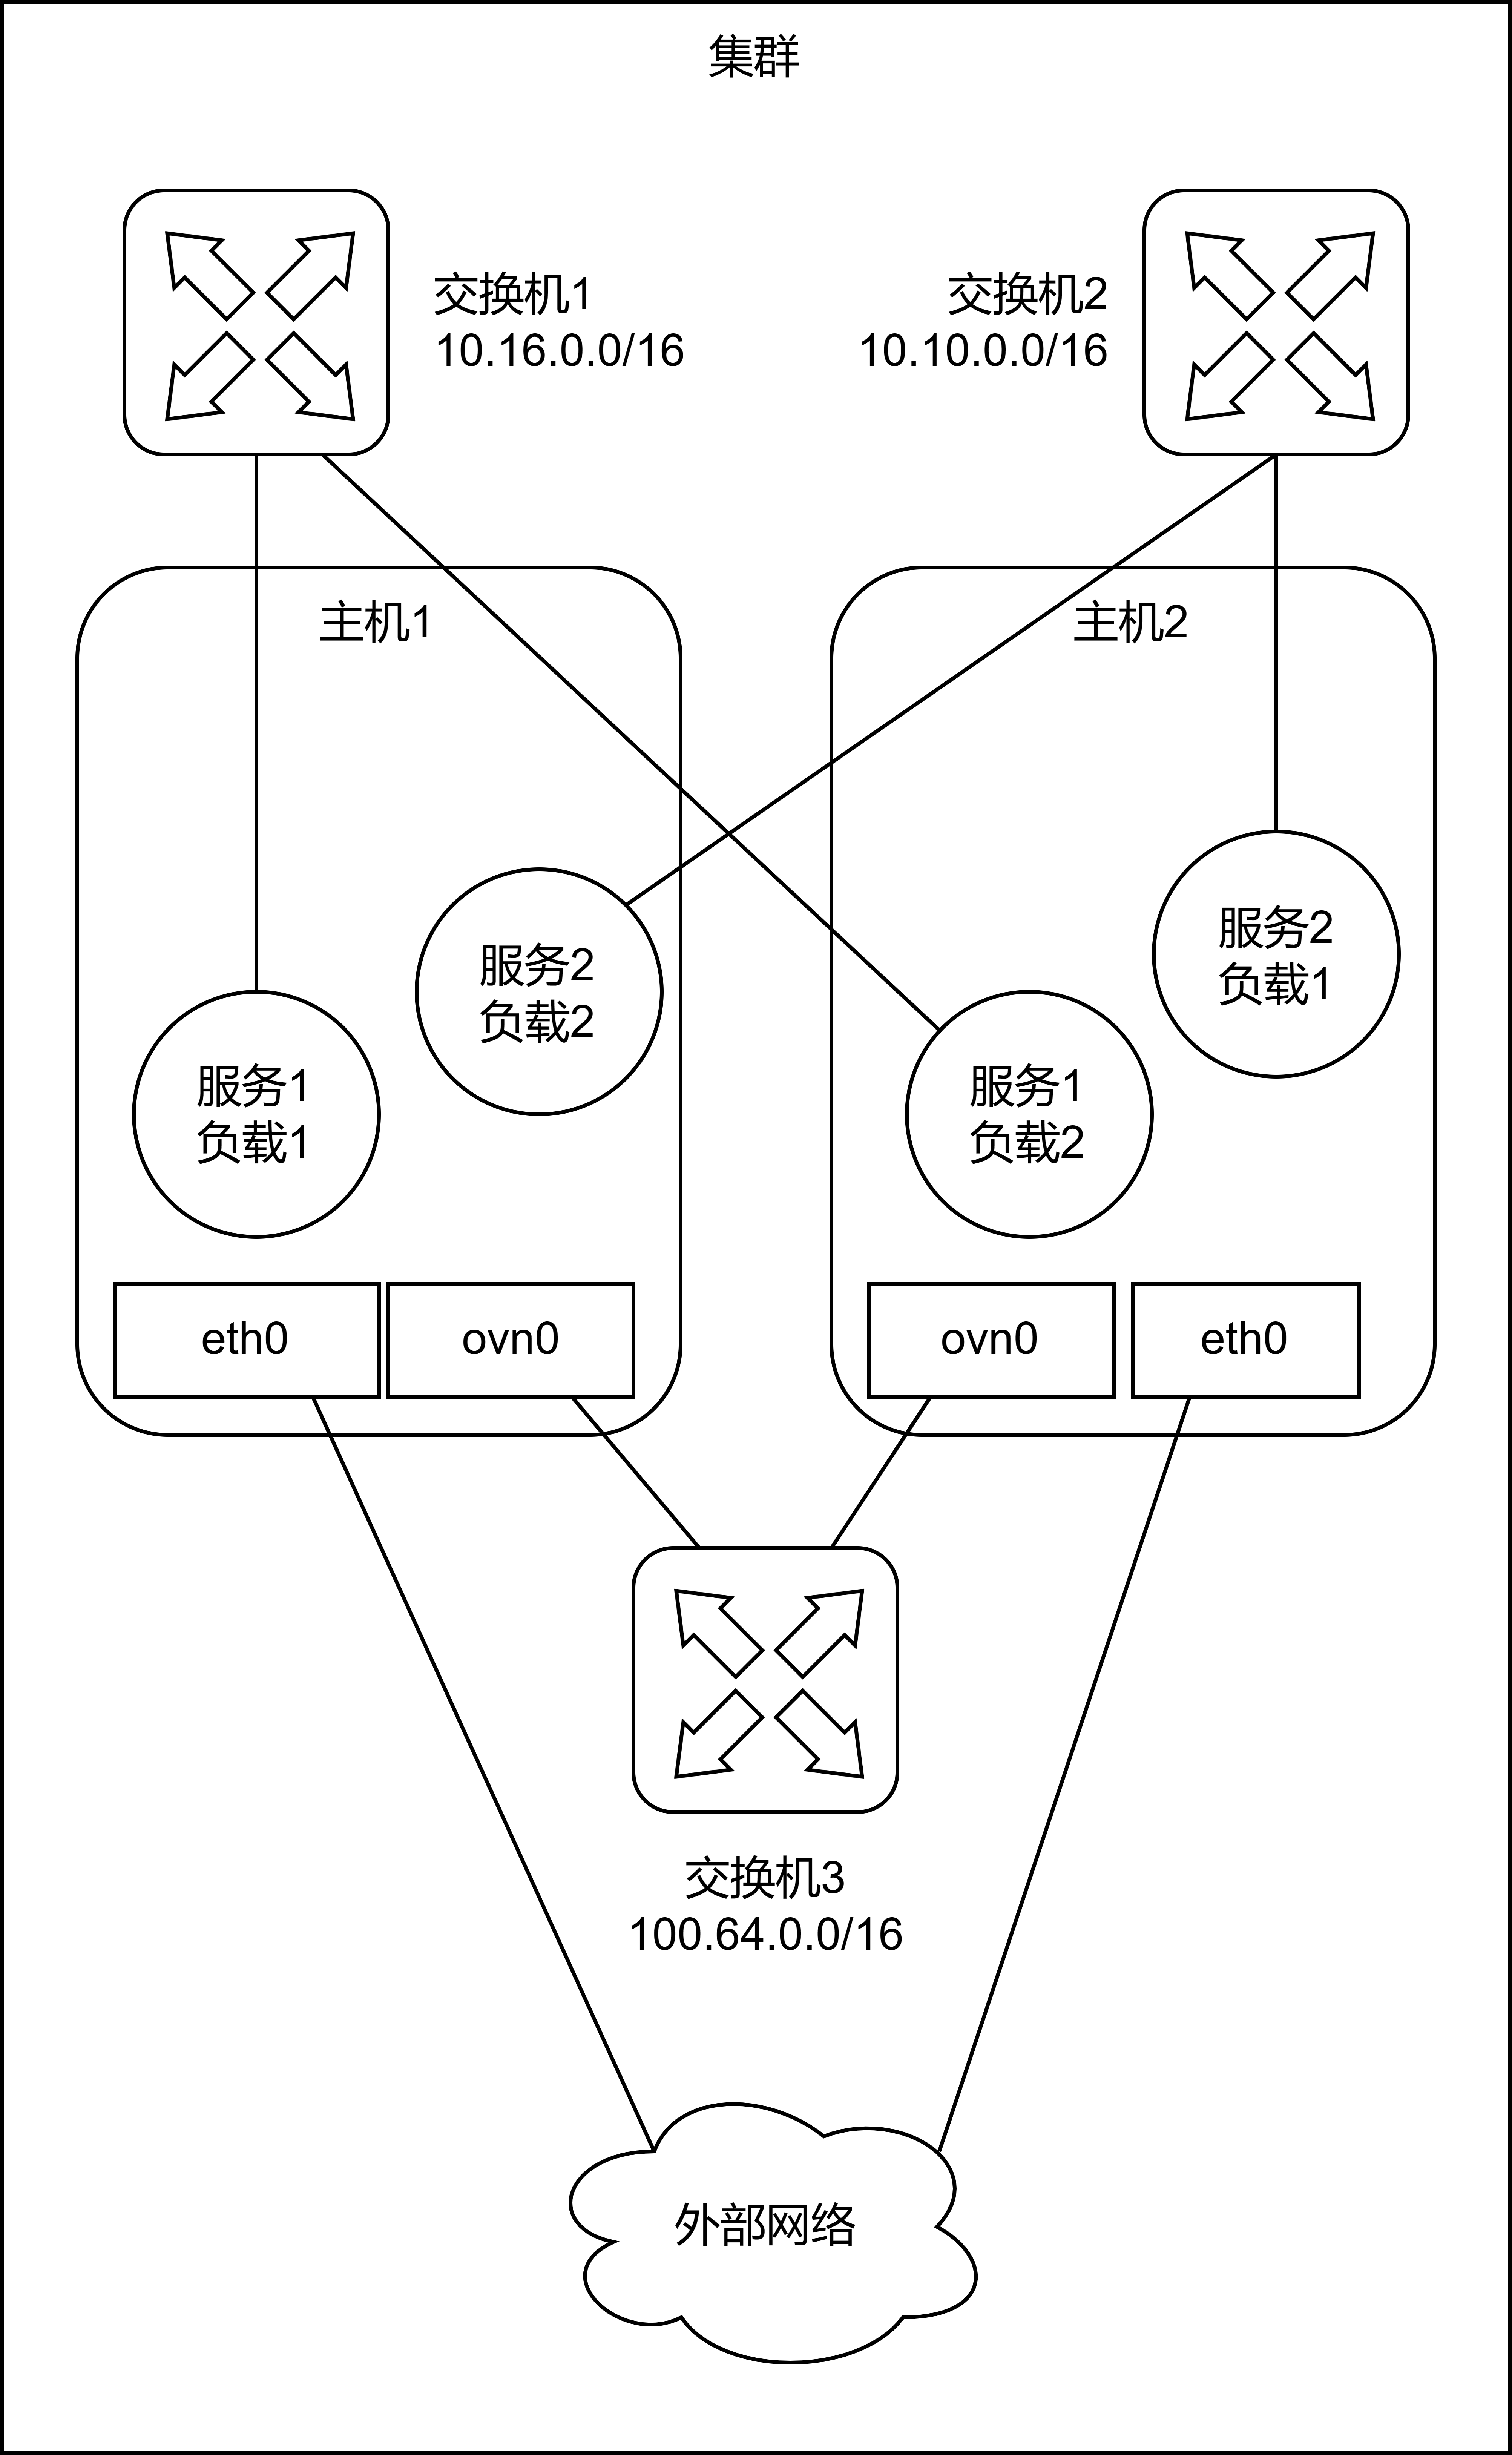
\includegraphics[width=0.50\textwidth]{networking-1}
%     \bicaption{\enspace Kubernetes-dataset 数据集网络拓扑结构}{\enspace Networking Topology of Kubernetes-dataset}
%     \label{fig:networking-1}

% \end{figure}

\begin{table}[t]
    \bicaption{\enspace Kubernetes-dataset 元数据}{\enspace Kubernetes-dataset metadata}
    \label{tab:dataset-metadata}
    \centering
    \footnotesize% fontsize
    \setlength{\tabcolsep}{4pt}% column separation
    \renewcommand{\arraystretch}{1.2}%row space 
    \begin{tabular}{lcccccccc}
        \hline
        流的数量 & 64 599\\
        良性流的数量 & 60 471\\
        ——其中:与攻击场景相关的良性流的数量 & 26 595\\
        恶意流的数量 & 4 128\\
        ——其中:与攻击场景相关的恶意流的数量 & 2 806\\
        ——其中:横向移动流的数量 & 163\\
        流的特征数量 & 79\\
        \hline
    \end{tabular}
\end{table}

}